\subsection{Rozpiętość i wielomian Jonesa} % (fold)
\label{sub:span}
\begin{conjecture}[Tait] \label{taitjones}  \index{Hipoteza Taita}
    Niech zorientowany splot $L$ posiada zredukowany, spójny, alternujący diagram o $n$ skrzyżowaniach.
    Wtedy każdy diagram ma co najmniej $n$ skrzyżowaniach.
\end{conjecture}

To bardzo ważny rezultat, którego prawdziwość przypuszczał już P. G. Tait w XIX wieku.
Nikt nie był w stanie podać dowodu przed pojawieniem się wielomianu Jonesa.
Dokonali tego Thistlethwaite, Kauffman oraz Murasugi w 1987 roku.
Wyjaśnimy teraz użyte tu przymiotniki.

\begin{definition}
Diagram jest zredukowany, gdy nie zawiera usuwalnych skrzyżowań:
\[
    \begin{tikzpicture}[baseline=-0.65ex,scale=0.07]
    \begin{knot}[clip width=5]
        \strand[semithick] (-5,-5) rectangle (5,5);
        \strand[semithick] (-5, -3) [in=right, out=left] to (-15, 3);
        \strand[semithick] (-5, 3) [in=right, out=left] to (-15, -3);

        \node at (-20, -3) {$\ldots$};
        \node at (-20,  3) {$\ldots$};
    \end{knot}
    \end{tikzpicture}
\]
\end{definition}

\begin{definition}
Diagram jest spójny, gdy nie można go podzielić na dwie niepuste części, które nie spotykają się na żadnym skrzyżowaniu.
\end{definition}

W dowodzie hipotezy Taita użyjemy rozpiętości wielomianu Jonesa.

\begin{definition}
    Rozpiętością wielomianu Laurenta $f$ jednej zmiennej $X$ nazywamy różnicę między najwyższym oraz najmniejszym wykładnikiem pojawiającym się w $f$: $\operatorname{span} f = M_f - m_f$.
\end{definition}

Zajmiemy się teraz wzorem pozwalającym na wyznaczenie nawiasu Kauffmana dowolnego splotu o $n$ skrzyżowaniach przez dodanie $2^n$ wyrazów (które odpowiadają digramom bez skrzyżowań).
Wzór ten okaże się użyteczny przy dowodzeniu późniejszych twierdzeń.

\begin{definition}
Niech $D$ będzie diagramem splotu.
\begin{enumerate}
\item \emph{Stan} $D$ to funkcja $s$ ze zbioru skrzyżowań $D$ w $\{-1, +1\}$.
\item Dla ustalonego stanu $s$ diagramu $D$ przez $sD$ rozumiemy diagram powstały przez wygładzenie
wszystkich skrzyżowań zgodnie z ich nowym znakiem ($\pm 1$), wtedy $|s|$ to suma wartości $s$.
\item Diagram dla $sD$ jest sumą zamkniętych krzywych, ich liczbę oznaczamy przez $|sD|$.
\end{enumerate}
\end{definition}

\begin{proposition}[o sumowaniu stanów]
Niech $D$ będzie diagramem splotu.
Wtedy
\[\langle D\rangle = \sum_s \underbrace{(-A^2-A^{-2})^{|sD|-1} A^{|s|}}_{\langle D \mid s \rangle},\]
gdzie sumujemy po wszystkich stanach $s$ dla $D$.
\end{proposition}

\begin{proof}
Oznaczmy prawą stronę dowodzonej równości przez $[D]$.
Pokażemy, że spełnia ona $[\LittleUnknot]=1$, $[D\sqcup\LittleUnknot]=(-A^{-2}-A^2) [D]$ oraz $[\LittleRightCrossing] = A [\LittleRightSmoothing] + A^{-1}[\LittleLeftSmoothing]$.
Stąd wynika już, że $[D] = \bracket{D}$.

Niewęzeł $\LittleUnknot$ ma tylko jeden stan $s$ z $|s| = 0$ i $|s\,\LittleUnknot| = 1$.

Zauważmy, że $D \sqcup \LittleUnknot$ i $D$ mają te same skrzyżowania,
więc możemy utożsamiać stany $s$ dla $D$ ze stanami $u$ dla $D \sqcup \LittleUnknot$.
Wtedy $|u| = |s|$ oraz $|u(D \sqcup \LittleUnknot)| = |sD| + 1$.
Zatem
\begin{align*}
    [D \sqcup \LittleUnknot]
    & = \sum_u (-A^2-A^{-2})^{|u(D\sqcup\LittleUnknot)|-1} A^{|u|} \\
    & = \sum_s (-A^2-A^{-2})^{|sD|} A^{|s|} = (-A^2-A^{-2}) [D].
\end{align*}

Pozostała trzecia własność. Z definicji $A[\LittleRightSmoothing]=\sum_u(-A^2-A^{-2})^{|u\LittleRightSmoothing|-1}A^{|u|+1}$,
gdzie $u$ przebiega wszystkie stany $\LittleRightSmoothing$.
Ale $\LittleRightSmoothing$ to $\LittleRightCrossing$ ze skrzyżowaniem (powiedzmy, $c$) wygładzonym dodatnio,
co daje bijekcję między stanami $u$ dla $\LittleRightSmoothing$ i $s$ dla $\LittleRightCrossing$, dla których $s(c) = + 1$.
Wtedy $|s\LittleRightCrossing|=|u\LittleRightSmoothing|$ i $|s|=|u|+1$ oraz
\[
A[\LittleRightSmoothing] = \sum_u (-A^2-A^{-2})^{|u\,\LittleRightSmoothing|-1}A^{|u|+1} = \sum_{s(c)=1}(-A^2-A^{-2})^{|s\,\LittleRightCrossing|-1}A^{|s|},
\]
podobne rozumowanie pokazuje, że $A^{-1}[\LittleLeftSmoothing] = \sum_{s(c)=-1}(-A^2-A^{-2})^{|s\,\LittleRightCrossing|-1}A^{|s|}$.
Teraz wystarczy dodać do siebie dwa ostatnie równania. %: $A[\PrawyGladki]+A^{-1}[\LewyGladki] = \sum_s(-A^2-A^{-2})^{|s\,\LittleRightCrossing|-1}A^{|s|} = [\RightCrossing]$.
\end{proof}

Zbadamy teraz dwa najprostsze stany dowolnego diagramu.

\begin{definition}
    Stan przypisujący znak $+ 1$ każdemu skrzyżowaniu nazywamy $s_+$.
    Analogicznie definiujemy $s_-$.
\end{definition}

Niech $D$ będzie alternującym, zredukowanym diagramem spójnym.
Wtedy wszystkie jego skrzyżowania mają ten sam znak.
Wybierzmy dla niego uszachowienie.
\[
    \begin{tikzpicture}[baseline=-0.65ex,scale=0.15]
    \begin{knot}[clip width=5]
        \strand[semithick] (-25, 0) to (25, 0);
        \strand[semithick] (10*0-15, -5) to (10*0-15, 5);
        \strand[semithick] (10*1-15, -5) to (10*1-15, 5);
        \strand[semithick] (10*2-15, -5) to (10*2-15, 5);
        \strand[semithick] (10*3-15, -5) to (10*3-15, 5);
        \draw[fill=blue!10!white,draw=none] (-25, 0) rectangle (-15, -5);
        \draw[fill=blue!10!white,draw=none] (-15, 0) rectangle (-5, 5);
        \draw[fill=blue!10!white,draw=none] (-5, 0) rectangle (5, -5);
        \draw[fill=blue!10!white,draw=none] (5, 0) rectangle (15, 5);
        \draw[fill=blue!10!white,draw=none] (15, 0) rectangle (25, -5);
        \node[above left] at (-15, 0) {$+1$};
        \node[above left] at (5, 0) {$+1$};
        \node[below left] at (-5, 0) {$+1$};
        \node[below left] at (15, 0) {$+1$};
    \end{knot}
    \end{tikzpicture}
\]

Zamieniając biały i czarny w razie potrzeby możemy założyć, że wszystkie skrzyżowania są dodatnie ($+1$).
Takie uszachowienie nazywamy \emph{standardowym}.
Porównajmy wygładzenie $s_+D$ z $s_-D$:
\[
    
\begin{tikzpicture}[baseline=-0.65ex,scale=0.10]
        \node at (0, 8) {$s_+D$};
        \draw[fill=blue!10!white,draw=none] (-25, -5) rectangle (25, 5);
        \draw[fill=white, draw=none] (-15, -5) [in=left, out=up] to (-12, 0) -- (-8, 0) [in=up, out=right] to (-5, -5);
        \draw[fill=white, draw=none] (5, -5) [in=left, out=up] to (8, 0) -- (12, 0) [in=up, out=right] to (15, -5);
        \draw[fill=white, draw=none] (-5, 5) [in=left, out=down] to (-2, 0) -- (2, 0) [in=down, out=right] to (5, 5);
        \draw[fill=white, draw=none] (-25, 0) -- (-18, 0) [in=down, out=right] to (-15, 5) -- (-25, 5);
        \draw[fill=white, draw=none] ( 25, 0) -- ( 18, 0) [in=down, out=left] to ( 15, 5) -- ( 25, 5);
    \end{tikzpicture}
    \quad
    
\begin{tikzpicture}[baseline=-0.65ex,scale=0.10]
        \node at (0, 8) {$s_-D$};
        \draw[fill=blue!10!white, draw=none] (-15, 5) [in=left, out=up] to (-12, 0) -- (-8, 0) [in=up, out=right] to (-5, 5);
        \draw[fill=blue!10!white, draw=none] (5, 5) [in=left, out=up] to (8, 0) -- (12, 0) [in=up, out=right] to (15, 5);
        \draw[fill=blue!10!white, draw=none] (-5, -5) [in=left, out=down] to (-2, 0) -- (2, 0) [in=down, out=right] to (5, -5);
        \draw[fill=blue!10!white, draw=none] (-25, 0) -- (-18, 0) [in=down, out=right] to (-15, -5) -- (-25, -5);
        \draw[fill=blue!10!white, draw=none] ( 25, 0) -- ( 18, 0) [in=down, out=left] to ( 15, -5) -- ( 25, -5);
    \end{tikzpicture}
\]

Zamknięte krzywe tworzące $s_+D$ są brzegami białych obszarów uszachowienia,
podczas gdy te tworzące $s_-D$ stanowią brzeg czarnych obszarów.
Zauważmy jeszcze, że na każdym skrzyżowaniu są cztery różne czarne i białe obszary
(nie mogą się spotkać w innych miejscach), gdyż diagram był zredukowany.

\begin{lemma}
Niech $D$ będzie spójnym diagramem splotu o $n$ skrzyżowaniach.
Wtedy mamy nierówność $|s_+D|+|s_-D|\le n+2$, z równością dla zredukowanego i alternującego $D$.
\end{lemma}

\begin{proof}
Skorzystamy z indukcji względem $n$.
Łatwo widać prawdziwość lematu dla $n = 0$.
Załóżmy, że jest on prawdziwy dla wszystkich diagramów o $n - 1$ skrzyżowaniach, następnie ustalmy diagram $D$ o $n$ skrzyżowaniach.

Wybierzmy skrzyżowanie z $D$. Można je wygładzić na dwa sposoby, jeden z nich daje spójny diagram $D'$.
Bez straty ogólności przyjmijmy, że jest to dodatnie wygładzenie.
Wtedy zachodzi $|s_+D'| = |s_+D|$, ale $|s_-D'|=|s_-D|\pm 1$, ponieważ $s_-D'$ powstaje z $s_-D$ przez zastąpienie pewnej części
$\LittleRightSmoothing$ z $\LittleLeftSmoothing$.
To rozrywa jedną krzywą na dwa kawałki lub scala dwie krzywe w jedną.
Teraz $|s_+D|+|s_-D| = |s_+D'|+|s_-D'|\pm 1 \le (n-1)+2\pm 1 \le n+2$ (pierwsza nierówność wynika z założenia indukcyjnego).

Załóżmy, że $D$ jest spójny, alternujący i zredukowany.
Musimy pokazać, że ostatnie dwie nierówności tak naprawdę są równościami.
Pierwsza wynika z tego, że $D'$ jest spójny, alternujący i zredukowany.
Z drugiej strony $|s_-D'|=|s_-D|-1$, ponieważ przejście od $s_-D$ do $s_-D'$ skleja dwa czarne obszary.
To pokazuje drugą równość i kończy dowód.
\[
    \begin{tikzpicture}[baseline=-0.65ex,scale=0.20]
    \begin{knot}[clip width=5]
        \strand[semithick] (-5, 0) to (5, 0);
        \strand[semithick] (0, -5) to (0, 5);
        \draw[fill=blue!10!white,draw=none] (-5, -5) rectangle (0, 0);
        \draw[fill=blue!10!white,draw=none] ( 5,  5) rectangle (0, 0);
        \node at (0, -8) {$D$};
    \end{knot}
    \end{tikzpicture}
    \quad
    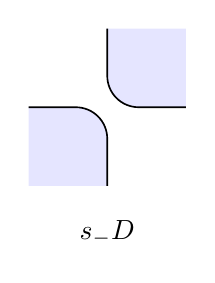
\begin{tikzpicture}[baseline=-0.65ex,scale=0.20]
        \draw[fill=blue!10!white, draw=none] (-5, 0) -- (-2, 0) [in=up, out=right] to (0, -2) -- (0, -5) -- (-5, -5);
        \draw[fill=blue!10!white, draw=none] (5, 0) -- (2, 0) [in=down, out=left] to (0, 2) -- (0, 5) -- (5, 5);
        \draw[semithick] (-5, 0) -- (-2, 0) [in=up, out=right] to (0, -2) -- (0, -5);
        \draw[semithick] (5, 0) -- (2, 0) [in=down, out=left] to (0, 2) -- (0, 5);
        \node at (0, -8) {$s_-D$};
    \end{tikzpicture}
    \quad
    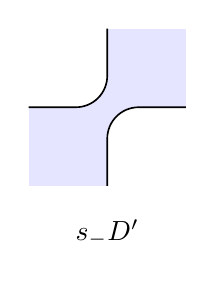
\begin{tikzpicture}[baseline=-0.65ex,scale=0.20]
        \draw[fill=blue!10!white, draw=none] (-5, -5) rectangle (5, 5);
        \draw[fill=white, draw=none] (5, 0) -- (2, 0) [in=up, out=left] to (0, -2) -- (0, -5) -- (5, -5);
        \draw[fill=white, draw=none] (-5, 0) -- (-2, 0) [in=down, out=right] to (0, 2) -- (0, 5) -- (-5, 5);
        \draw[semithick] (5, 0) -- (2, 0) [in=up, out=left] to (0, -2) -- (0, -5);
        \draw[semithick] (-5, 0) -- (-2, 0) [in=down, out=right] to (0, 2) -- (0, 5);
        \node at (0, -8) {$s_-D'$};
    \end{tikzpicture}
    \qedhere
\]
\end{proof}
\begin{lemma}
Niech $D$ będzie diagramem splotu o $n$ skrzyżowaniach.
Wtedy
\begin{enumerate}
\item $M \langle D \rangle \le n+2|s_+D|-2$
\item $m \langle D \rangle \ge -n-2|s_-D|+2$
\end{enumerate}
z równością, jeżeli $D$ jest alternujący, zredukowany i spójny.
\end{lemma}

\begin{proof}
Udowodnimy tylko pierwszą część, druga jest do niej podobna.
Oznaczymy przez $\langle D \mid s \rangle$ wielkość $(-A^{-2}-A^2)^{|sD|-1}A^{|s|}$.
Zauważmy, że $M\langle D|s\rangle=2|sD|+|s|-2$,
a więc w szczególności $M\langle D|s_+\rangle=2|s_+D|+n-2$.
Gdyby udało się nam pokazać, że $M\langle D|s\rangle \le M\langle D|s_+\rangle$
dla wszystkich innych stanów $s$, dowód nierówności byłby zakończony.
Ale możemy znaleźć ciąg $s_+ = s_0$, $s_1$, \ldots, $s_r=s$,
w którym $s_{i+1}$ powstaje z $s_i$ przez pojedynczą zmianę $+1$ na $-1$.

Teraz $|s_{i+1}|=|s_i|-2$, podczas gdy $|s_{i+1}D|=|s_iD|\pm 1$,
ponieważ $s_{i+1}D$ uzyskujemy z $s_{i}D$ przez połączenie dwóch zamkniętych krzywych lub podział jednej zamkniętej krzywej na dwie części.
Zatem
\begin{align*}
    M \langle D \mid s_{i+1} \rangle & =
    2|s_{i+1}D|+|s_{i+1}|-2 \\ & =
    (2|s_iD| + |s_i| -2 ) + (\pm 2-2) \le
    M \langle D|s_i\rangle.
\end{align*}

Widać już, że $M\langle D \mid s\rangle =M\langle D \mid s_r\rangle \le\ldots\le M\langle D \mid s_0\rangle=M\langle D \mid s_+\rangle$.

Pokażemy teraz, że jeśli $D$ jest zredukowany, alternujący i spójny, to nierówność zamienia się w równość.
Będzie to wynikało z  $M\langle D|s\rangle<M\langle D| s_+\rangle$
dla $s\neq s_+$, jeżeli tylko powołamy się na powyższy argument.
Wystarczy ograniczyć się do tych $s$, które powstają z $s_+$ przez zmianę pojedynczego stanu $+1$ na $-1$.
Ale to już jest oczywiste, gdyż $sD$ otrzymujemy przez sklejenie dwóch białych obszarów $s_+ D$.
\end{proof}

Możemy wreszcie zająć się rozpiętością wielomianu Jonesa.

\begin{theorem}
Niech $L$ będzie zorientowanym splotem o spójnym diagramie $D$ z $n$ skrzyżowaniami.
Wtedy $\operatorname{span}(V(L)) \le n$, z równością dla zredukowanego i alternującego $D$.
\end{theorem}

\begin{proof}
    Pokażemy prawdziwość innego, równoważnego stwierdzenia: $\operatorname{span} \langle D\rangle\le 4n$
    z równością dla zredukowanego i alternującego $D$.
    Dwa poprzednie lematy mówią, że
    \begin{align*}
        \operatorname{span}\langle D\rangle
        & = M\langle D\rangle - m\langle D\rangle \le (2|s_+D|+n-2)+(2|s_-D|+n-2) \\
        & = 2(|s_+D|+|s_- D|)+2n-4 \le 2(n+2)+2n-4 = 4n. \qedhere
    \end{align*}
\end{proof}

Jesteśmy już w stanie podać dowód twierdzenia \ref{taitjones} wspomnianego na początku sekcji.

\begin{proof}
    Założenia mówią nam, że $\operatorname{span} (V(L)) = n$.
    Gdyby istniał diagram o mniejszej liczbie skrzyżowań,
    mielibyśmy $\operatorname{span} (V(L)) < n$, co prowadzi do sprzeczności.
\end{proof}

Szukanie wielomianu Jonesa splotu bywa uciążliwe,
jednak czasami możemy oszacować jego rozpiętość korzystając z następujących nierówności:

\begin{corollary}
    Niech $L$ będzie zorientowanym splotem ze spójnym diagramem $D$ o $n$ skrzyżowaniach.
    Wtedy
    \begin{align*}
        3w(D)-2|s_+D|+2-n & \le 4 m(V(L) \\
        3w(D)+2|s_-D|+n-2 & \ge 4 M(V(L)),
    \end{align*}
    z równością dla zredukowanego i alternującego $D$.
\end{corollary}

\begin{proof}
    Proste ćwiczenie.
\end{proof}

% Koniec podsekcji Rozpiętość i wielomian Jonesa
